\section{Experiments}
\subsection{Experiment Details}
We ran the tests on a laptop using the Criterion benchmarking tool for haskell. The graphs were generated using Criterions ability to output data to csv. Each test was run for each queue type, n times. The values of n that was used went from 500 to 10000 with gaps of 500.

\subsubsection{Test Types}
Four types of tests was done:
\begin{description}
\item{1. \texttt{test\_pop}}
This test pops n elements off the queue. This test tells us something about how a lot of pops on the four different queues effects running time.
\item{2. \texttt{test\_inject}}
This test inject n elements onto the queue and tells us something about the effect of inject on running time.
\item{3. \texttt{test\_pop\_inject}}
In this test we pop an element from the queue and inject another. This is done n times.
\item{4. \texttt{test\_repeated\_inject\_pop}}
Here we repeatedly inject some element to the same queue while popping an element as well to make it not be optimized away. n elements are injected into the queue.
\end{description}



\subsection{Expectations}
When comparing the 4 different queue implementations, we expect them to perform as follow:
\begin{description}

\item[1. Haskell List:]
The Haskell List queue implementation performs \texttt{inject} in $O(n)$ time, and as such, we expect it to perform horribly on any test case that requires pushes.
On pure \texttt{pop} operations however, it will be $O(1)$, with a very low overhead, and as such it will most likely be among the fastest queues at performing \texttt{pop}s.
\item[2. Paired O(1) Non-Reusable Queue:]
The Paired Queue implementation should be fairly low-overhead, and as such perform quite well, except on the special test case, where we reuse queues.
\item[3. Real-Time Strict Queues:] 
The Real-Time Strict Queue should generally perform well on all test cases, since we have a nice $O(1)$ worst-case guarentee for all operations. This queue however, has quite a large overhead, and will therefore most likely be outperformed by most other queues in tests cases where they exhibit $O(1)$ performance. 
\item[4. Lazy Amortized $O(1)$ Queues:]
The Lazy Queue should perform very well on all test cases. Not only does it have $O(1)$ amortized cost for all operation, it also has quite a low overhead. 

\end{description}

\subsection{Computer Specs:}
\begin{tabular}{| r  l |} \hline
Model: &  ASUS 1215N \\ \hline
OS: & Ubuntu 12.10 \\ \hline
CPU: & Intel Atom Dual Core 1.8GHz\\ \hline
Memory: & 2 GB\\ \hline
\end{tabular}

\subsection{Result}
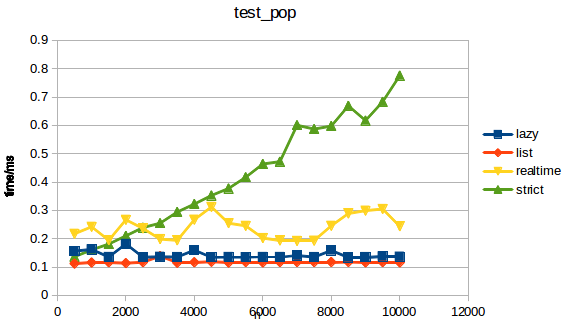
\includegraphics{Graphs/test_pop.png}


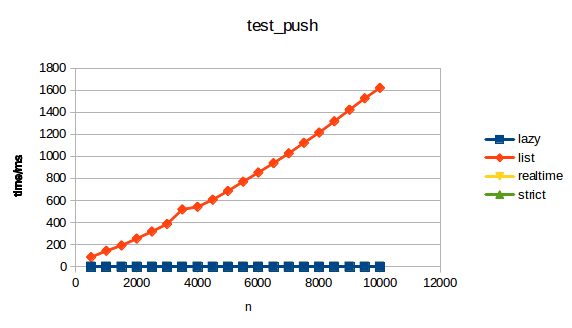
\includegraphics{Graphs/test_push.png}


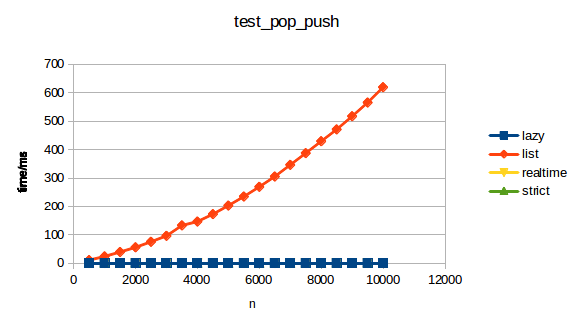
\includegraphics{Graphs/test_pop_push.png}


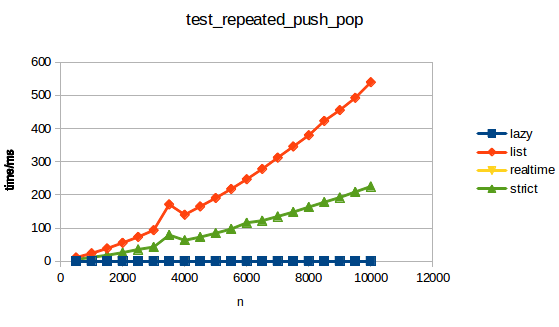
\includegraphics{Graphs/test_repeated_push_pop.png}


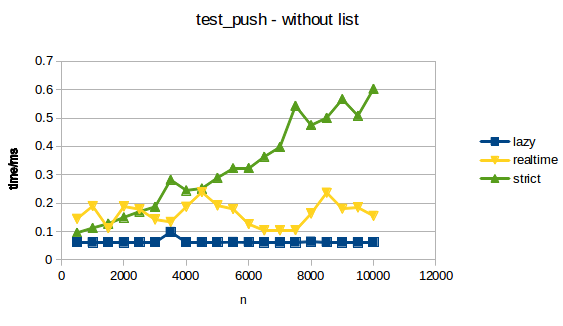
\includegraphics{Graphs/test_push_without_list.png}


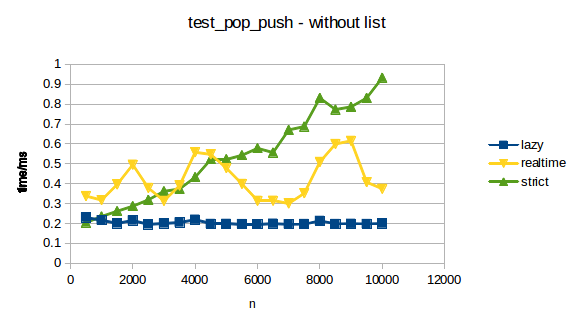
\includegraphics{Graphs/test_pop_push_without_list.png}


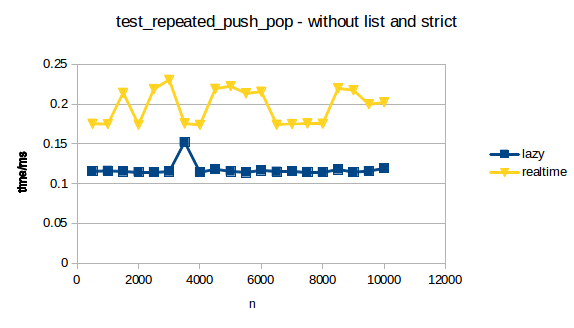
\includegraphics{Graphs/test_repeated_push_pop_without_list.png}


\subsection{Test Conclusions}
 
From the test results, we can conclude the following about the 4 different queues;

\begin{description}
\item[1. Haskell List:]
We see that the simple list-based data structure performs very well on \texttt{pop}, outperforming all the other data structures.
However, on any test involving \texttt{inject}, the queue quickly slows down, due to the $O(n)$ cost of adding new items to the queue. 

\item[2. Paired O(1) Non-Reusable Queue:]
The Paired Queue shows some interesting behaviour.
First of all, we note that the data structure seems to be slightly linear in the size of the queue on all operations. This is most due to the fact that a very large reversed end list will build up as the data structure is constructed, leading to an $O(n)$ reversal on the first \texttt{pop}. Not that this also happens on the \texttt{inject} test case, as a single \texttt{pop} is performed to force thunks.

We can also clearly see the problems of the queue when reusing the data structure, which makes the queue perform and $O(n)$ operation for each pop.

\item[3. Real-Time Strict Queues:] 
The Real-Time Strict Queues show $O(1)$ performance on every operation, though we note that they are considerably slower than their lazy counterpart.

\item[4. Lazy Amortized $O(1)$ Queues:]
The Lazy Queues seem to not only be quite fast, but also maintain an almost constant speed, as opposed to the Real-Time queues, whose performance seem to vary somewhat.
\end{description}
